Chapter~\ref{chap:memo15} introduced two atomic controllers that enforced
desired safety properties when run separately. That chapter also described
how to compose components, but informally followed the convention that
components being composed do not constrain overlapping sets of
variables. However, such a restriction is natural in sampled-data systems,
for example when composing two controllers outputing to the same sets of
actuators. This raises the question: when can two such controllers be run
in parallel in order to enforce the conjunction of their respective safety
properties? More generally, when can a sampled-data system be built up
modularly from smaller components while ensuring the properties guaranteed
by each of the components and avoiding inconsistencies in the composed
system? This chapter provides a series of proof rules to address that
question.

As alluded to above, one of the challenges is in ensuring that the
specification of the discrete controller is always enabled, i.e. it always
specifies at least one successor state.  While this might seem trivial,
consider the following scenario.  Suppose we have built a module that
prevents a quadcopter from exceeding some maximum altitude.  Furthermore,
suppose we have also built another module that prevents the quadcopter from
violating some \emph{minimum} altitude.  If we have separately verified
that these two modules enforce their respective properties, we would like
to compose them in parallel to guarantee both properties simultaneously.
That is, we would like the composed system to guarantee that the system
never goes too high or too low.  However, this is not always possible; a
module could enforce the upper bound on altitude by always accelerating
downwards.  Likewise, a module could enforce the lower bound on altitude by
always accelerating upwards.  Clearly, na\"ively composing the controllers
of these modules in parallel would result in a system that gets stuck --
there is never an acceleration that both controllers can agree on.

In this chapter, we present sound techniques for resolving this and other
potential pitfalls for reusing and composing modules for sampled-data
systems.  We observed that modularity is facilitated by separating
verification into two parts: \emph{preservation} and \emph{\progress{}}.
Preservation ensures that the model guarantees the safety property
inductively, while \progress{} ensures that the system model is always
enabled.  This separation facilitates the application of several simple,
general, and powerful operators, namely substitution, conjunction, and
disjunction.  More precisely, we state sufficient conditions for applying
these operators to individual modules to produce a new sampled-data system
with the desired properties (e.g. the conjunction of the safety properties
of conjoined modules).  Crucially, these sufficient conditions are in terms
of preservation and \progress{}.

To validate the expressiveness of our theorems, as in the rest of the
dissertation we apply them in the context of \emph{quadcopters}, by showing
how to compose several simple verified controllers together in different
ways to produce many different verified composed controllers.  To ensure
that our controllers are practical, we run them on an actual quadcopter.
In summary, the contributions of this chapter are:
\begin{itemize}
\setlength\itemsep{0.01em}
\item We implement in the Coq proof assistant a general approach for modular verification of sampled-data systems by separately exposing proofs of preservation and \progress{}. The development is available from the project webpage: \url{http://veridrone.ucsd.edu}.
\item We apply this approach to build and verify arbitrary 3D geofences for a quadcopter, including walls, boxes, and rectangular donuts, starting with two simple verified 1D controllers.
We show that our modular verification techniques keep the proof burden manageable.
\item We evaluate our geo-fences by running them on an actual quadcopter, and show that they work in practice.
\item We discuss the capabilities of three state-of-the-art fully-automated tools (SpaceEx, Flow*, and dReach) in verifying our geo-fence controllers.
\end{itemize}

\section{Overview}
We start with an informal description of the operators that our theory
covers: substitution, conjunction, and disjunction.  We then give an
overview of verifying controllers using these operators.  Finally, we
describe how we applied this to build a verified family of geo-fences for a
quadcopter.

\paragraph*{Operators}
\emph{Substitution} of expressions for variables represents a form of
reuse, allowing us to transform systems and their properties into a
different coordinate system.  For example, given a model of a system
defined in the x-y plane, the substitution $\{\tlavar{x} \mapsto \tlavar{r}
\cos \tlavar{\roll},\; \tlavar{y} \mapsto \tlavar{r} \sin \tlavar{\roll}\}$
transforms the model to polar coordinates, the substitution $\{\tlavar{x}
\mapsto \tlavar{y},\; \tlavar{y} \mapsto \tlavar{x}\}$ rotates the system,
and the substitution $\{\tlavar{x} \mapsto \tlavar{x} + 5\}$ translates the
system by 5 units in the $\tlavar{x}$ dimension.  However, not all
substitutions soundly transport both systems \emph{and} their properties;
our theory (Section~\ref{sec:subst}) gives formal conditions under which
substitutions are permitted.

\emph{Disjunction} of two systems represents nondeterministic choice
between the controllers of the system.  For example, if we have a
controller that prevents a quadcopter from flying too far to the west and
another controller that prevents a quadcopter from flying too far north,
then their disjunction enforces a north-west no-fly zone -- the quadcopter
must stay to the north \emph{or} to the west of the no-fly zone.  Unlike
conjunction, there is no risk of the composed system getting stuck.
Instead, the challenge with disjunction is in constraining the
nondeterministic choice between the controllers.  Our theorems and
definitions in Section~\ref{sec:disjunctive-composition} make this formal
by including the inductive invariants of each system within the composed
controller.

\emph{Conjunction} of two systems represents parallel composition of these
systems.  For example, if we have a system that enforces an upper bound on
velocity and a system that enforces a lower bound on velocity, then their
conjunction enforces both an upper and a lower bound on velocity.  We can
also conjoin systems that control or restrict different variables, such as
a system that enforces a bound on velocity and a system that enforces a
bound on position.  However, as discussed in the introduction, the
challenge of applying this operator is in ensuring that the conjoined
systems never get stuck, e.g. when the controller of one system requires
positive acceleration while the other requires negative acceleration.
Again, our theory (Section~\ref{sec:conjunctive-composition}) gives formal
conditions under which conjunctive composition is possible.

Note that disjunctive and conjunctive composition are related to
alternative and parallel composition.

\paragraph*{Controller Verification}
To illustrate how the operators work, we explain the construction and
modular verification of several general purpose controllers for enforcing
state constraints, depicted in Figure~\ref{fig:library}.  We begin with a
simple verified module: a controller that enforces an upper bound on
position in one spatial dimension by controlling acceleration (depicted by
(a) in Figure~\ref{fig:library}).  We use substitution to ``mirror'' this
module and its correctness property, thus obtaining a module (b) that
enforces a lower bound on position, again in one dimension.  We conjoin
these two modules to form a controller (c) enforcing upper and lower bounds
on position, still in one dimension.  We use substitution to rotate this
interval controller into a second, orthogonal dimension (d), then conjoin
(c) and (d) to form a controller (e) enforcing a 2 dimensional rectangle,
i.e. upper and lower bounds on position in two dimensions.  Finally, we use
substitution to build and verify four translated copies of (e) and
disjunction of these four copies to enforce a rectangular donut (f).  We
use disjunction to enforce that the system must, at all times, be in the
first copy of (e), the second, the third, \emph{or} the fourth.  Moreover,
since the rectangles are overlapping, the system can transition from one
rectangle to another.

\begin{figure}[t]
  \centering
  \begin{tikzpicture}
    \tikzstyle{every node}=[fill=black!15,node distance=0.5cm,font=\scriptsize]
    \tikzstyle{every path}=[draw=black,ultra thick]

   \node[draw=none,minimum height=0.65cm,minimum width=0.65cm,label=left:{(a)}] (y+) at (-2,2) {}
     (\tikzlastnode.north west)edge(\tikzlastnode.north east);

   \node[draw=none,minimum height=0.65cm,minimum width=0.65cm,label=right:{(b)}] (y-) at (2,2) {}
     (\tikzlastnode.south west)edge(\tikzlastnode.south east);

   \def\aoff{0.1};

   \draw[-latex,thick] ($(y+.east) + (\aoff,0)$) -- ($(y-.west) - (\aoff,0)$)
     node[draw=none,fill=none,font=\scriptsize,midway,above] {substitution};

   \def\coffx{0.35};
   \def\coffy{0.45};

   \node[draw=none,minimum height=0.65cm,minimum width=0.65cm,label=left:{(c)}] (y+-) at (-2,0.55) {}
     (\tikzlastnode.north west)edge(\tikzlastnode.north east)
     (\tikzlastnode.south west)edge(\tikzlastnode.south east)
     node[fill=none] at ($(y+-.north east) +(\coffx,\coffy)+(0.1,0)$) {conjunction};

   \draw[-latex,thick] ($(y+.south)-(0,\aoff)$) -- ($(y+-.north) + (0,\aoff)$);
   \draw[-latex,thick] (y-) -- (y+-);

   \node[draw=none,minimum height=0.65cm,minimum width=0.65cm,label=right:{(d)}] (x+-) at (2,0.55) {}
     (\tikzlastnode.north west)edge(\tikzlastnode.south west)
     (\tikzlastnode.north east)edge(\tikzlastnode.south east);

   \draw[-latex,thick] ($(y+-.east) + (\aoff,0)$) -- ($(x+-.west) - (\aoff,0)$)
     node[draw=none,fill=none,font=\scriptsize,midway,above] {substitution};

   \node[draw=black,ultra thick,minimum height=0.65cm,minimum width=0.65cm,label=left:{(e)}] (xy+-) at (-2,-1) {}
     node[fill=none] at ($(xy+-.north east) +(\coffx,\coffy)+(0.1,0)$) {conjunction};

   \draw[-latex,thick] ($(y+-.south) - (0,\aoff)$) -- ($(xy+-.north) + (0,\aoff)$);
   \draw[-latex,thick] (x+-) -- (xy+-);

   \node[draw=black,ultra thick,minimum height=1.5cm,minimum width=1.5cm,label=right:{(f)}] (donut_out) at (2,-1) {};
   \node[draw=black,ultra thick,fill=white,minimum height=0.5cm,minimum width=0.5cm] (donut_in) at (2,-1) {};
   \node[draw=black,thick,dashed,fill=none,minimum height=0.5cm,minimum width=1.5cm] (donut1) at (2,-0.5) {};
   \node[draw=black,thick,dashed,fill=none,minimum height=0.5cm,minimum width=1.5cm] (donut2) at (2,-1.5) {};
   \node[draw=black,thick,dashed,fill=none,minimum height=1.5cm,minimum width=0.5cm] (donut3) at (2.5,-1) {};
   \node[draw=black,thick,dashed,fill=none,minimum height=1.5cm,minimum width=0.5cm] (donut4) at (1.5,-1) {};

   \draw[-latex,thick] (xy+-.east) -- (donut1.center);
   \draw[-latex,thick] (xy+-) -- (donut2.center)
     node[draw=none,fill=none,font=\scriptsize,pos=0.4,below,text width=2cm] {substitution and disjunction};
   \draw[-latex,thick] (xy+-) edge[thick,out=0,in=170] (donut3.center);
   \draw[-latex,thick] (xy+-) -- (donut4.center);

  \end{tikzpicture}

     \caption{Overview of construction and verification of position bounding controllers.}
     \label{fig:library}
\end{figure}

\paragraph*{Quadcopter}
Although the above approach can enforce state constraints for a variety of
applications (e.g. trains, intelligent cruise control), we evaluate our
approach in the context of \emph{quadcopter} controllers that enforce
position and velocity bounds.  We performed this verification modularly
starting from two simple verified modules that we ported from prior work:
one enforcing an upper bound on velocity and another enforcing an upper
bound on position, both in one spatial dimension.  Connecting the
verification methodology above to quadcopters required application of the
three operators under the complex, coupled dynamics of a quadcopter, thus
showcasing the applicability of our rules to solve complex problems.
Crucially, our Coq theorems for each of these operators give formal
conditions under which this is sound.

Ultimately, we were able to use the verification techniques in
Figure~\ref{fig:library} to build a three dimensional bounding box of both
position and velocity for the quadcopter.  This bounding cube provides a
powerful building block for constructing ``pixelated shapes'' (analogous to
(f) in Figure~\ref{fig:library}), which can be used to enforce interesting
shapes such as a flying around and over but not near the pilot.  The
results of our verification along with actual flight tests are in
Section~\ref{sec:eval}.  A primary takeaway is that substitution,
conjunction, and disjunction are powerful operations that can take simple
controllers verified with respect to simple dynamics and turn them into
controllers that enforce complex constraints in complex dynamics.

\section{A Modular Basis for Reasoning}
\label{sec:compositional-basis}
In this section, we present the framework that we use for modular reasoning
about sampled-data systems: separating proofs into preservation and
\progress{}.  This foundation will allow us to build the theory for
applying substitution, conjunction, and disjunction (presented in
Section~\ref{sec:compositional-monitors}).  We start by formally
illustrating the difficulty of modular reasoning in this domain. We use the
notation and definitions from Chapter~\ref{chap:prelim}. As a small note,
throughout this section when $X$ is a system, we use $\D_X$ and $\W_X$ to
denote the discrete and continuous transitions of $X$, respectively.  Also,
we use the inductive invariant of a system as its initial condition; thus
we use $I$ to denote an inductive invariant and $I_X$ to denote the
inductive invariant of system $X$.  In practice, one must prove that the
initial condition of a system implies the inductive invariant.

\subsection{Stuck Specifications}
The physical world always evolves because time always evolves.
Cyber-physical system specifications should adhere to this property -- the
specification should never reach a state in which it is stuck, i.e. in
which a transition is impossible.  For example, consider the system
$\Sys{\mathsf{False}}{\W}{\Delta}$.  In this system, there is never a
discrete transition (expressed using the unsatisfiable action formula
$\mathsf{False}$).  Since a discrete transition never occurs, a continuous
transition is not possible once time reaches $\Delta$.  Readers familiar
with Zeno specifications~\cite{abadi1994realtime} will note that \SysA{}
specifications that are never stuck are non-Zeno.

We rule out such specifications using a new abstraction called \System,
defined as follows:
\[
\SystemP{D}{\W}{\Delta} \triangleq \Sys{D}{\W}{\Delta} \vee \neg \EnabledP{\big(\Sys{D}{\W}{\Delta}\big)}
\]
In the above, \Enabled takes an action formula and returns a state formula.
In particular, $\Enabled (A)$ holds on a given state $st$ iff there exists
a next state $st'$ such that $(st, st')\in A$, i.e. the system can take an
$A$ transition.  A specification whose transition is built using \System
can never become stuck; if the underlying \SysA{} becomes stuck (not
\Enabled), then the clause $\neg \EnabledP{\big(\Sys{D}{\W}{\Delta}\big)}$
conservatively expresses that anything can happen.  Informally, we will not
be able to prove any interesting global properties of a \System when the
underlying \SysA{} can reach a state in which it is not \Enabled since we
will know nothing about the next state.

It may seem trivial to avoid writing stuck specifications for sampled-data
systems, and thus the distinction between \SysA{} and \System appears to be
only theoretical.  However, avoiding stuck specifications is a core
challenge of building sampled-data systems modularly. To see why, consider
the following. In general, our end goal is to prove properties of the form:
\[
\entails I \wedge \Always (\SystemP{D}{\W}{\Delta}) \rightarrow \Always S
\]
This property states that, starting with initial condition $I$, condition
$S$ always holds if at each point in the trace, the transition relation is
described by $(\SystemP{D}{\W}{\Delta})$.  Unfortunately, properties like
the one above are not modular.  For example, suppose we have two discrete
transitions $D_1$ and $D_2$ which independently ensure $S_1$ and $S_2$,
i.e.
\[
\vdash I \wedge \Always (\SystemP{D_1}{\W}{\Delta}) \rightarrow \Always S_1
\]
\[
\vdash I \wedge \Always (\SystemP{D_2}{\W}{\Delta}) \rightarrow \Always S_2
\]
We would like to combine these proofs to show that $S_1~\wedge~S_2$ is an
invariant of the conjoined system \SystemP{(D_1 \wedge D_2)}{\W}{\Delta}.
Unfolding the definition of \System reveals that this is not, in general,
true.  The problem is that $\EnabledP{D_1} \wedge \EnabledP{D_2}$ does not
necessarily imply $\EnabledP{(D_1 \wedge D_2)}$ (Consider
\EnabledP{(\tlavar{x}\tlaprime = 1~\wedge~\tlavar{x}\tlaprime = 0)}).
This means that the following two formulas are not necessarily equivalent:
\[
\SystemP{D_1}{\W}{\Delta}\wedge\SystemP{D_2}{\W}{\Delta}
\]
\[
\SystemP{(D_1 \wedge D_2)}{\W}{\Delta}
\]
This formalizes the challenge described in the introduction -- na\"ive
parallel composition (conjunction) of controllers can result in a
controller that gets stuck.

Crucially, \Enabled is inherently non-modular, so global invariant proofs
of systems specified using \System are inherently non-modular. By ruling
out stuck specifications, we also rule out the modularity of \emph{global}
invariant proofs.

\subsection{Regaining Modularity}
The key to regaining modularity is a shift from global proofs to local
ones.  In particular, we will make the inductive invariant of the system
explicit and use it to prove two properties independently: preservation of
the invariant, and progress of the system under the invariant.  As we will
see in Section~\ref{sec:compositional-monitors}, this decomposition of the
global property into local ones makes it much easier to combine and re-use
systems and their proofs.

\paragraph{Preservation}
Preservation of property ($I$) under an action formula states if $I$ holds
in the current state then it holds in the next state. Formally,
\[
\SysPreservesP{I}{\big(\SysP{D}{\W}{\Delta}\big)} \;\triangleq\; I \wedge \mathsf{Sys}_{\mathsf{inv}} \wedge \SysP{D}{\W}{\Delta} \rightarrow I\tlaprime
\]
where $I\tlaprime$ represents the state formula $I$ with all variables
primed.  The $\mathsf{Sys}_{\mathsf{inv}}$ premise expresses the invariants
guaranteed by the \SysA{} abstraction, namely that no more than $\Delta$
time elapses between discrete transitions.

\paragraph{\Progress{}}
Progress under an invariant justifies that the system is \Enabled assuming
the invariant. Formally,
\[\begin{array}{l}
\SysNeverStuckP{I}{\left(\Sys{D}{\W}{\Delta}\right)} \triangleq \\
\qquad I \wedge \mathsf{Sys}_{\mathsf{inv}} \rightarrow \EnabledP{\left(\Sys{D}{\W}{\Delta}\right)}
\end{array}
\]
This condition allows us to prove that a \SysA{} and a \System{} describe
exactly the same system.

Note that, here, progress is a safety property that is closely related to
the notion of progress in programming languages.  It is different than
progress properties in distributed systems, and it is different than
convergence to an equilibrium in control theory.

\paragraph{Combining Preservation \& \Progress{}}
Preservation of and \progress{} under the \emph{same} inductive invariant
is sufficient to prove that the invariant is a global invariant of the
corresponding \System, which is ultimately our goal.  This is captured by
the following theorem:

\begin{theorem}{\ProofRule{LocalToGlobal}}
\[\begin{array}{rl}
 & \SysPreservesP{I}{\left(\Sys{D}{\W}{\Delta}\right)} \\
\wedge & \SysNeverStuckP{I}{\left(\Sys{D}{\W}{\Delta}\right)} \\
\wedge & I \rightarrow S \\
\vdash & I \wedge \Always \left(\SystemP{D}{\W}{\Delta}\right) \rightarrow \Always S
\end{array}
\]
\end{theorem}

\section{Modular Sampled-data Systems}
\label{sec:compositional-monitors}

In this section, we show how to use preservation and \progress{} to reason
modularly about sampled-data systems.  In particular, for each of our three
operators (substitution, disjunction, and conjunction), we present theorems
that state formal conditions under which application of the operator
guarantees preservation and \progress{}.  We illustrate each of the
operators and corresponding theorems by building verified
state-constraining controllers for quadcopters.  This allows us to
construct and verify controllers enforcing policies such as ``do not fly
above 400 feet'' (FAA regulation for recreational drones), ``do not fly
within 5 miles of an airport'', and ``do not fly within 5 feet of the
pilot.''

It is important to note that all of the state-constraining controllers that
we verify are \emph{non-deterministic}.  This means that the discrete
transitions do not compute a single value for each control variable
(e.g. acceleration) but instead describe a set of allowed values that
ensure the desired state-constraint.  As we will see, this non-determinism
is crucial for conjunctive composition
(Section~\ref{sec:conjunctive-composition}).  In Section~\ref{sec:eval}, we
discuss how the actual implementation of these controllers resolves this
non-determinism.

\paragraph{Building blocks}
As the basic building blocks of our development, we start with the two
sampled-data systems that are minor variants on the ones from
Chapter~\ref{chap:memo15}. Both operate in one spatial dimension, i.e.
\[\begin{array}{rcl}
\W_{1D} & \triangleq & \dt{\tlavar{y}} = \tlavar{v} \wedge \dt{\tlavar{v}} = \tlavar{a} \wedge \dt{\tlavar{a}} = 0
\end{array}
\]
The two controllers each enforce constant bounds on a state variable by
controlling acceleration (\tlavar{a}).  The first-derivative controller
(\derivShimv) bounds velocity using acceleration (the first-derivative of
velocity).  The second-derivative controller (\derivShimx) bounds position
using acceleration (the second-derivative of position).  To ensure that
\derivShimx{} can stop before violating the boundary, the controller is
parameterized by \Tmin which represents the braking acceleration and
smallest possible acceleration (and is negative).
Figure~\ref{fig:formal-monitors} gives the discrete transitions and
inductive invariants for the two systems. Each inductive invariant states
that, given the time until the next discrete transition, the system can
stop before the boundary.


\begin{figure}[t]

\textbf{First-Derivative Controller} ($\derivShimv = \Sys{D_\partial}{W_{1D}}{\Delta}$)
\[\begin{array}{rl}
D_\partial \triangleq & \Ca\tlaprime \wedge (\tlanextvar{a} \cdot \Delta + \tlavar{v} \leq ub \vee \tlanextvar{a} \leq 0) \\
\invShimv \triangleq & (\tlavar{a} < 0 \rightarrow \tlavar{v} \leq ub) \wedge
(\tlavar{a} \geq 0 \rightarrow \tlavar{a} \cdot \tlavar{\tau} + \tlavar{v} \leq ub) \\
\end{array}
\]

\textbf{Second-Derivative Controller} ($\derivShimx = \Sys{D_{\partial^2}}{W_{1D}}{\Delta}$)
\[
\begin{array}{rl}
D_{\partial^2} \triangleq & (0 \leq \tlavar{v} + \tlanextvar{a} \cdot \Delta \rightarrow \\
& \;\quad \tdist{\tlavar{v}}{\tlanextvar{a}}{\Delta} + \sdist{\tlavar{v} + \tlanextvar{a}\cdot\Delta} + \tlavar{y} \leq \ubY) \\
& (\tlavar{v} + \tlanextvar{a} \cdot \Delta \leq 0 \wedge 0 < \tlavar{v} \rightarrow \\
& \;\quad \tdist{\tlavar{v}}{\tlanextvar{a}}{\frac{-\tlavar{v}}{\tlanextvar{a}}} + \tlavar{y} \leq \ubY) \wedge \Ca\tlaprime \\
\invShimx \triangleq & \forall t : \mathbb{R}, 0 \leq t \leq \tlavar{\tau} \rightarrow \\
& \;\quad \tlavar{\Y} {+} \tdist{\tlavar{\V}}{\tlavar{a}}{t} + \sdist {\max(0,\tlavar{\V} + \tlavar{a} \cdot t)} \leq \ubY
\end{array}
\]
\[
\begin{array}{ccc}
\tdist{\V}{a}{\Delta} \triangleq \V\cdot\Delta+\frac{a\cdot\Delta^2}{2} & \qquad &
\sdist{\V} \triangleq -\frac{\V^2}{2\cdot a_{\mathsf{min}}} \\
\Ca \triangleq \amin \leq \tlavar{a} & \qquad & \amin  < 0
\end{array}
\]

\caption{Discrete transitions and inductive invariants for our building blocks.}
\label{fig:formal-monitors}
\end{figure}

In Chapter~\ref{chap:memo15}, we verified variants on both of these
controllers in a global style but did \emph{not} compose them.  For the
work in this chapter, we ported each of the global proofs to our local,
modular specification by extracting the inductive invariant (which was
stated explicitly in the proof) and the preservation proof (which formed
the inductive case).  Beyond extracting the safety proofs, we also had to
verify \progress{}, which was not addressed in Chapter~\ref{chap:memo15},
but is trivial for such basic modules.  In the remainder of this section,
we denote the preservation and \progress{} proofs of the two controllers
by: \ProofRule{$\partial$-Preserves},
\ProofRule{$\partial$-\xmakefirstuc{\progress{}}},
\ProofRule{$\partial^2$-Preserves}, and
\ProofRule{$\partial^2$-\xmakefirstuc{\progress{}}}.

\paragraph{Quadcopter Controller}
\label{sec:quadcopter-dynamics}
To build and verify controllers for quadcopters, we need a model of the
physical dynamics of a quadcopter, called $\W_{QC}$:
\[\begin{array}{rl}
\W_{QC} \triangleq & \left(\begin{array}{ll}
       & \dt{\tlavar{x}} = \tlavar{v_x} \wedge \dt{\tlavar{y}} = \tlavar{v_y} \wedge \dt{\tlavar{z}} = \tlavar{v_z} \\
\wedge & \dt{\tlavar{v_x}} = \tlavar{T} \cos \tlavar{\roll} \sin \tlavar{\pitch} \\
\wedge & \dt{\tlavar{v_y}} = -\tlavar{T} \sin \tlavar{\roll} \\
\wedge & \dt{\tlavar{v_z}} = \tlavar{T} \cos \tlavar{\roll} \cos \tlavar{\pitch} - g \\
\wedge & \dt{\tlavar{\roll}} = 0 \wedge \dt{\tlavar{\pitch}} = 0 \wedge \dt{\tlavar{T}} = 0
\end{array}\right)
\end{array}
\]

\begin{figure}
\centering

\newcommand{\rotateRPY}[4][0/0/0]% point to be saved to \savedxyz, roll, pitch, yaw
{   \pgfmathsetmacro{\rollangle}{#2}
   \pgfmathsetmacro{\pitchangle}{#3}
   \pgfmathsetmacro{\yawangle}{#4}

   % to what vector is the x unit vector transformed, and which 2D vector is this?
   \pgfmathsetmacro{\newxx}{cos(\yawangle)*cos(\pitchangle)}% a
   \pgfmathsetmacro{\newxy}{sin(\yawangle)*cos(\pitchangle)}% d
   \pgfmathsetmacro{\newxz}{-sin(\pitchangle)}% g
   \path (\newxx,\newxy,\newxz);
   \pgfgetlastxy{\nxx}{\nxy};

   % to what vector is the y unit vector transformed, and which 2D vector is this?
   \pgfmathsetmacro{\newyx}{cos(\yawangle)*sin(\pitchangle)*sin(\rollangle)-sin(\yawangle)*cos(\rollangle)}% b
   \pgfmathsetmacro{\newyy}{sin(\yawangle)*sin(\pitchangle)*sin(\rollangle)+ cos(\yawangle)*cos(\rollangle)}% e
   \pgfmathsetmacro{\newyz}{cos(\pitchangle)*sin(\rollangle)}% h
   \path (\newyx,\newyy,\newyz);
   \pgfgetlastxy{\nyx}{\nyy};

   % to what vector is the z unit vector transformed, and which 2D vector is this?
   \pgfmathsetmacro{\newzx}{cos(\yawangle)*sin(\pitchangle)*cos(\rollangle)+ sin(\yawangle)*sin(\rollangle)}
   \pgfmathsetmacro{\newzy}{sin(\yawangle)*sin(\pitchangle)*cos(\rollangle)-cos(\yawangle)*sin(\rollangle)}
   \pgfmathsetmacro{\newzz}{cos(\pitchangle)*cos(\rollangle)}
   \path (\newzx,\newzy,\newzz);
   \pgfgetlastxy{\nzx}{\nzy};

   % transform the point given by #1
   \foreach \x/\y/\z in {#1}
   {   \pgfmathsetmacro{\transformedx}{\x*\newxx+\y*\newyx+\z*\newzx}
       \pgfmathsetmacro{\transformedy}{\x*\newxy+\y*\newyy+\z*\newzy}
       \pgfmathsetmacro{\transformedz}{\x*\newxz+\y*\newyz+\z*\newzz}
       \xdef\savedx{\transformedx}
       \xdef\savedy{\transformedy}
       \xdef\savedz{\transformedz}
   }
}

\tikzset{RPY/.style={x={(\nxx,\nxy)},y={(\nyx,\nyy)},z={(\nzx,\nzy)}}}

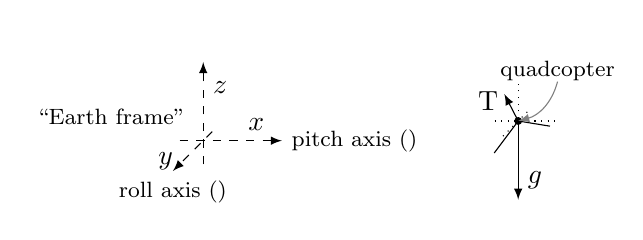
\begin{tikzpicture}

 \begin{scope}[yshift=-0.75cm]
 \draw[-latex,dashed] (-0.3,0,0) to node[near end,above] {$x$} (1,0,0) node[right] {\footnotesize pitch axis (\tlavar{\pitch})} ;
 \draw[-latex,dashed] (0,-0.3,0) to node[near end,right] {$z$} (0,1,0) ;
 \draw[-latex,dashed] (0,0,-0.3) to node[near end,left] {$y$} (0,0,1) node[below] {\footnotesize roll axis (\tlavar{\roll})} ;
 \node[anchor=east] at (-0.1,0.3,0) {\footnotesize ``Earth frame''} ;
 \end{scope}

 \rotateRPY{30}{-20}{0}

 \begin{scope}[xshift=4cm,yshift=-0.5cm]

   \draw[dotted] (-0.3,0,0) -- (0.5,0,0) ;
   \draw[dotted] (0,-0.3,0) -- (0,0.5,0) ;
   \draw[dotted] (0,0,-0.3) -- (0,0,0.5) ;

   \begin{scope}[RPY]
   \draw (0,0,0) to (0.5,0,0) ;
   \draw[-latex] (0,0,0) to node[near end,left] {\tlavar{T}} (0,0.5,0) ;
   \draw (0,0,0) to (0,0,0.5) ;
   \fill[black] (0,0,0) circle (0.05cm) ;
   \end{scope}

   \draw[latex-,gray] (0,0,0) to[bend right] (0.5,0.5) node[inner sep=0.1,anchor=south,black] {\footnotesize quadcopter} ; 

   \draw[-latex] (0,0,0) to node[near end,right] {$g$} (0,-1,0) ;
 \end{scope}

\end{tikzpicture}


\caption{Free-body diagram and dynamics of the quadcopter.}
\label{fig:free-body}
\end{figure}

Here \tlavar{T} represents the combined thrust of the motors (normalized
with respect to the mass of the quadcopter), \tlavar{\pitch} represents the
pitch (the angle around the $y$-axis), and \tlavar{\roll} represents the
roll (the angle around the $x$-axis). Figure~\ref{fig:free-body} depicts
this graphically in a free-body diagram. Our model is based on the
simplifying assumption (called the ``small angle condition'') that a
trusted attitude controller can instantaneously achieve any pitch and roll
within the bounds $-30\mydegree$ to $30\mydegree$ with a thrust greater
than or equal to 0, while holding yaw constant at 0.
\[
\smallangle \triangleq \left| \tlavar{\pitch} \right| \leq 30\mydegree \wedge \left|\tlavar{\roll}\right| \leq 30\mydegree \wedge 0 \leq \tlavar{T}
\]
Prior work has suggested that this is a reasonable approximation under this
small-angle condition ($\smallangle$), since the attitude dynamics are
significantly faster than the velocity and position
dynamics~\cite{Gillula2011}.  We capture this condition by requiring that
all quadcopter controllers are enabled under $\smallangle$.  That is, our
goal is to build controllers $D$ such that
\[
\begin{array}{l}
\SysPreservesP{I}{(\Sys{(D\wedge\Next{\smallangle})}{\W_{QC}}{\Delta})}~\wedge \\
\SysNeverStuckP{I}{(\Sys{(D\wedge\Next{\smallangle}))}{\W_{QC}}{\Delta})}
\end{array}
\]

For some state-constraints and their corresponding controllers, it is only
necessary to reason about an abstraction of the quadcopter dynamics
$\W_{QC}$.  For example, reasoning about a controller that enforces a bound
on the vertical position \tlavar{z} might only require reasoning about the
portion of the dynamics on which \tlavar{z} depends.  We formalize this
with:
\[\begin{array}{rl}
 & \SysPreservesP{I}{(\Sys{(D\wedge\Next{\smallangle}))}{\W}{\Delta})}~\wedge \\
 & \SysNeverStuckP{I}{(\Sys{(D\wedge\Next{\smallangle})}{\W}{\Delta})} \\
 & (\W_{QC} \rightarrow \W)~\wedge \\
\entails & \SysPreservesP{I}{(\Sys{(D\wedge\Next{\smallangle})}{\W_{QC}}{\Delta})}~\wedge \\
 & \SysNeverStuckP{I}{(\Sys{(D\wedge\Next{\smallangle})}{\W_{QC}}{\Delta})}
\end{array}
\]
where $\W_{QC} \rightarrow \W$ states that $\W$ is an abstraction of
$\W_{QC}$.
